\documentclass[aspectratio=169,10pt]{beamer}
\usetheme{default}
\usecolortheme{default}
\setbeamertemplate{navigation symbols}{}
\setbeamertemplate{footline}[frame number]
\definecolor{epic}{RGB}{20,60,120}
\setbeamercolor{frametitle}{fg=epic}
\setbeamercolor{title}{fg=epic}
\setbeamercolor{structure}{fg=epic}
\setbeamerfont{frametitle}{size=\large,series=\bfseries}
\usepackage{booktabs}
\usepackage{amsmath,amssymb}
\usepackage{graphicx}
\graphicspath{{../../results/}}
\newcommand{\code}[1]{\texttt{\detokenize{#1}}}
\newcommand{\good}[1]{\textcolor{green!45!black}{#1}}
\newcommand{\bad}[1]{\textcolor{red!70!black}{#1}}

\title{$\Lambda\to p\pi^-$ in the ePIC B0 tracker: update}
\subtitle{Hit seeding (EICrecon\#3116), the 5\,keV default, and $\Lambda$s up to 275\,GeV}
\author{Gadi Ninio}
\date{12 November 2026}

\begin{document}

\begin{frame}
\titlepage
\centering\footnotesize Code, results, reports: \url{https://github.com/gadininio/eic-B0-detector}\\
Previous slides: \code{docs/slides/slides.pdf} (3 November 2026)
\end{frame}

%-------------------------------------------------------------------------------------
\begin{frame}{Reminder and what changed since 3 November}
\textbf{Reminder:} single-$\Lambda$ gun, $\theta = 8$--18\,mrad; $\Lambda\to p\pi^-$ reconstructed in the B0 tracker;
old B0 (epic \code{43f427e}, 300\,$\mu$m) vs realistic B0 of eic/epic\#1194 (\code{ec774d8}, 50\,$\mu$m);
truth-seeded tracks, EICrecon main \code{8b44cae}, 50--100\,GeV.
\vspace{2mm}
\small
\begin{tabular}{@{}p{0.2\textwidth}p{0.33\textwidth}p{0.42\textwidth}@{}}
\toprule
& 3 November & now\\
\midrule
B0 seeding & truth (\#2901) & truth \textbf{and hit seeding (\#3116)}, same job, same events\\
EICrecon & main \code{8b44cae} & \#3116 branch \code{1ca147b} (main of 11-11 + \#3116)\\
B0 threshold & 10\,keV default, 5\,keV by option & \good{5\,keV default} (EICrecon\#3084)\\
eic-shell & nightly 11-02 & nightly 11-07 (new B0 in its epic)\\
old geometry & from the container & local build of the same commit\\
$p_\Lambda$ & 50--100\,GeV & 50--100 (same events) \textbf{+ 100--275\,GeV}\\
\bottomrule
\end{tabular}
\vspace{2mm}
\begin{itemize}\small
\item \#3028 (first B0 seeding PR) closed 11-05 in favour of \#3116 (open); \#3029 was a bot fix into the \#3028 branch, not main
\end{itemize}
\end{frame}

%-------------------------------------------------------------------------------------
\begin{frame}{Hit seeding (EICrecon\#3116)}
\begin{itemize}
\item ACTS triplet seeder: one hit in each of \textbf{3 B0 stations}
\item Hits rotated so the dipole field at the middle hit is along $z$
\item No vertex or charge assumption $\Rightarrow$ works for displaced decays; min.\ $p$ across the field 1\,GeV, $\ge 3$ measurements
\item \code{B0TrackerSeeds} $\to$ \code{B0TrackerCKFTracks} $\to$ \code{CombinedTracks} $\to$ \textbf{\code{ReconstructedChargedParticles}}
\item Truth-seeded chain runs in parallel: \code{ReconstructedTruthSeededChargedParticles}
\item Seed $\leftrightarrow$ daughter: $\ge 2$ of the 3 seed hits made by the daughter
\item Macros: new argument \code{seeding = "truth" | "hit"}
\end{itemize}
\end{frame}

%-------------------------------------------------------------------------------------
\begin{frame}{Tracking efficiency: truth vs hit seeding (50--100\,GeV)}
\centering\small
\begin{tabular}{@{}lcccc@{}}
\toprule
accepted daughters, p / $\pi^-$ & old, truth & old, hit & new, truth & new, hit\\
\midrule
accepted & 404 / 349 & 404 / 349 & 295 / 240 & 295 / 240\\
seed & 99 / 99\,\% & \good{100 / 100\,\%} & 97 / 96\,\% & \good{100 / 100\,\%}\\
CKF track & 98 / 66\,\% & 100 / \bad{74\,\%} & 94 / 61\,\% & 100 / \bad{67\,\%}\\
\textbf{reconstructed particle} & \textbf{97.5 / 66.5\,\%} & \textbf{99.5 / 72.5\,\%} & \textbf{93.2 / 60.8\,\%} & \textbf{100 / 64.6\,\%}\\
\bottomrule
\end{tabular}
\vspace{3mm}
\begin{itemize}
\item Hit seeding: a seed for \textbf{every} accepted daughter, \textbf{every} accepted proton reconstructed
\item The $\pi^-$ is still lost in the \textbf{CKF}: 5--10\,GeV $\pi^-$ 39\,\% (new), 48\,\% (old) with hit seeding\\
$\Rightarrow$ \textbf{the soft-$\pi^-$ loss is not a seeding problem}
\end{itemize}
\end{frame}

%-------------------------------------------------------------------------------------
\begin{frame}{Tracking efficiency, new geometry}
\begin{columns}[T]
\column{0.5\textwidth}\centering truth seeding\\
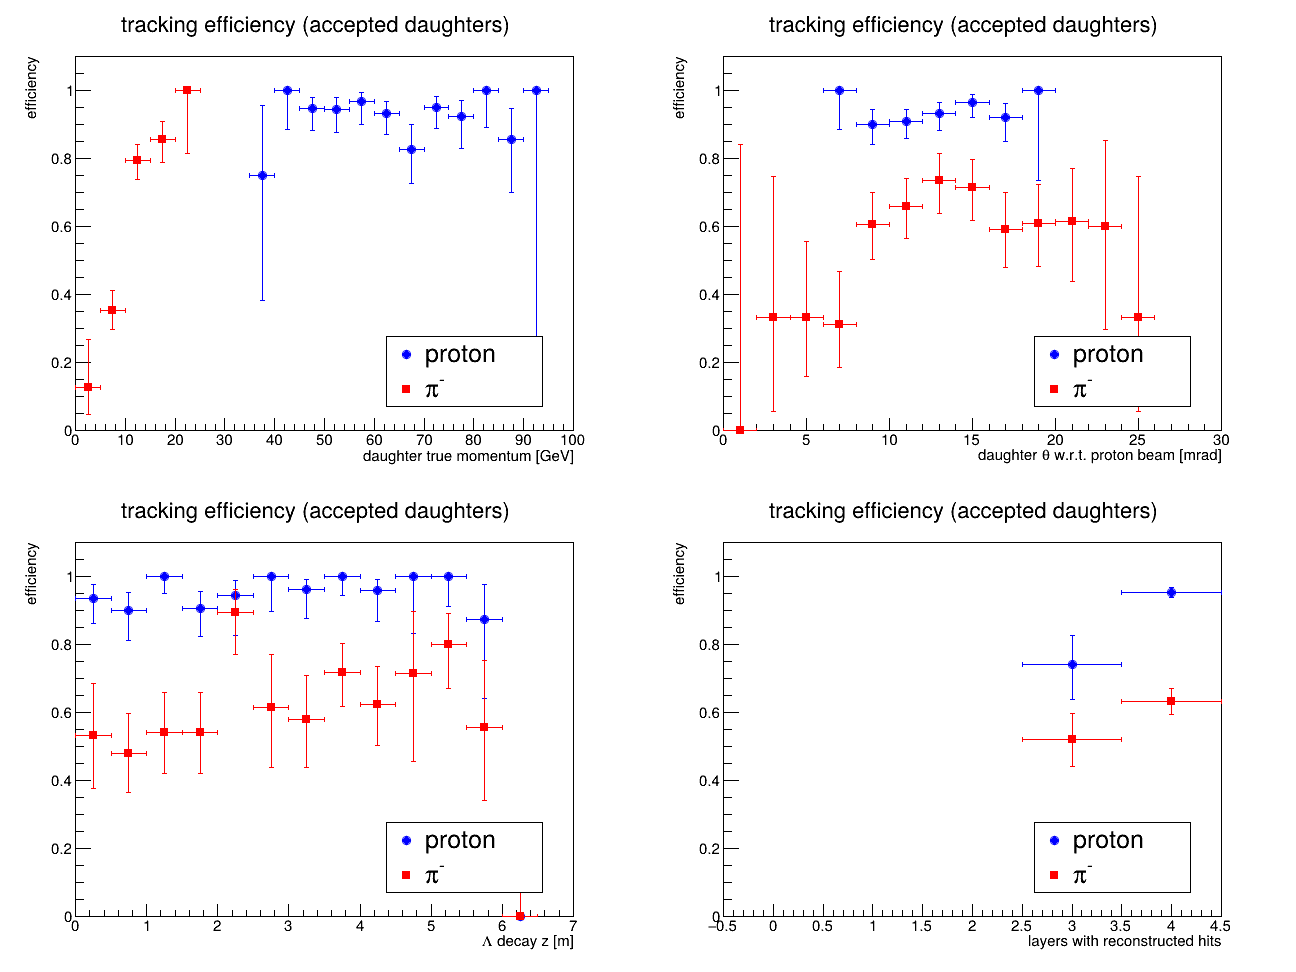
\includegraphics[width=\textwidth]{07_hit_seeding/tracking_efficiency_new_truth.png}
\column{0.5\textwidth}\centering hit seeding\\
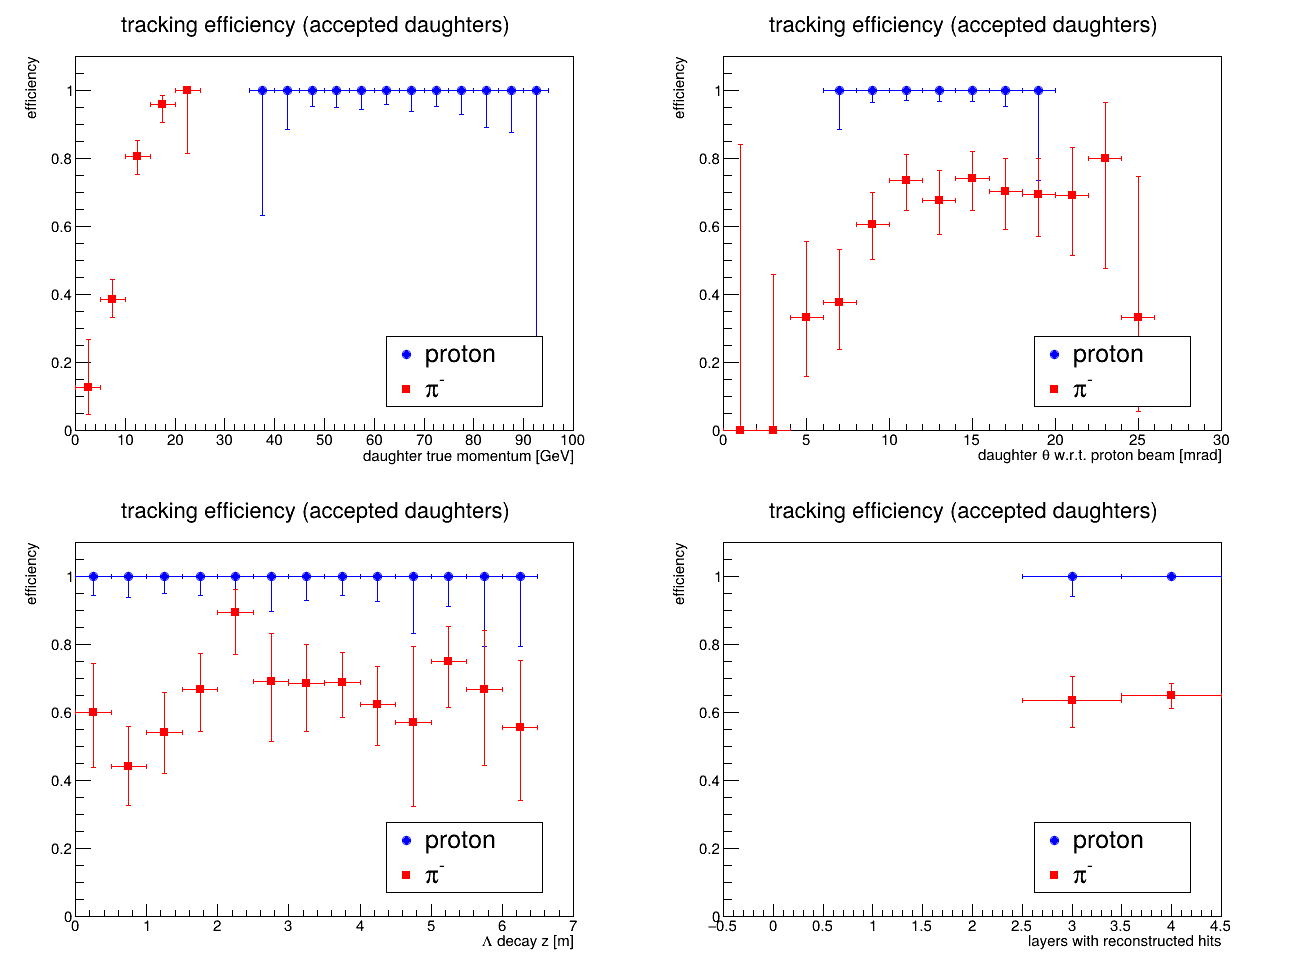
\includegraphics[width=\textwidth]{07_hit_seeding/tracking_efficiency_new_hit.png}
\end{columns}
\small vs daughter momentum, $\theta$, decay $z$, layers with rec.\ hits; proton blue, $\pi^-$ red
\end{frame}

%-------------------------------------------------------------------------------------
\begin{frame}{Acceptance $\times$ efficiency: 3 November vs now}
\centering\small
\begin{tabular}{@{}lccc@{}}
\toprule
& 3 Nov: main, truth & \#3116 build, truth & \#3116 build, \textbf{hit}\\
\midrule
\multicolumn{4}{@{}l}{\emph{old geometry}}\\
tracking eff.\ p / $\pi^-$ & 82.2 / 55.6\,\% & \bad{97.5 / 66.5\,\%} & 99.5 / 72.5\,\%\\
$A\times\varepsilon$ both / $p\pi^-$ decay & 29.8\,\% & \bad{41.7\,\%} & 45.5\,\%\\
both rec.\ / generated $\Lambda$ & 15.0\,\% & 21.0\,\% & \textbf{22.9\,\%}\\
\midrule
\multicolumn{4}{@{}l}{\emph{new geometry} (3 Nov: 5\,keV by option)}\\
tracking eff.\ p / $\pi^-$ & 92.9 / 60.8\,\% & 93.2 / 60.8\,\% & 100 / 64.6\,\%\\
$A\times\varepsilon$ both / $p\pi^-$ decay & 24.7\,\% & 24.7\,\% & 27.0\,\%\\
both rec.\ / generated $\Lambda$ & 12.0\,\% & 12.0\,\% & \textbf{13.1\,\%}\\
\bottomrule
\end{tabular}
\vspace{2mm}
\begin{itemize}\small
\item New geometry: truth seeding reproduces 3 November exactly; hit seeding \good{+1.1 points}
\item \bad{Old geometry, not understood:} same simulation, truth seeding, efficiency jumps with the new build.
Differences: EICrecon \code{8b44cae} $\to$ \code{1ca147b}, eic-shell image (ACTS), local epic build. Not the threshold
\end{itemize}
\end{frame}

%-------------------------------------------------------------------------------------
\begin{frame}{$\Lambda$ mass: truth vs hit seeding (same events)}
\begin{columns}[T]
\column{0.55\textwidth}\centering
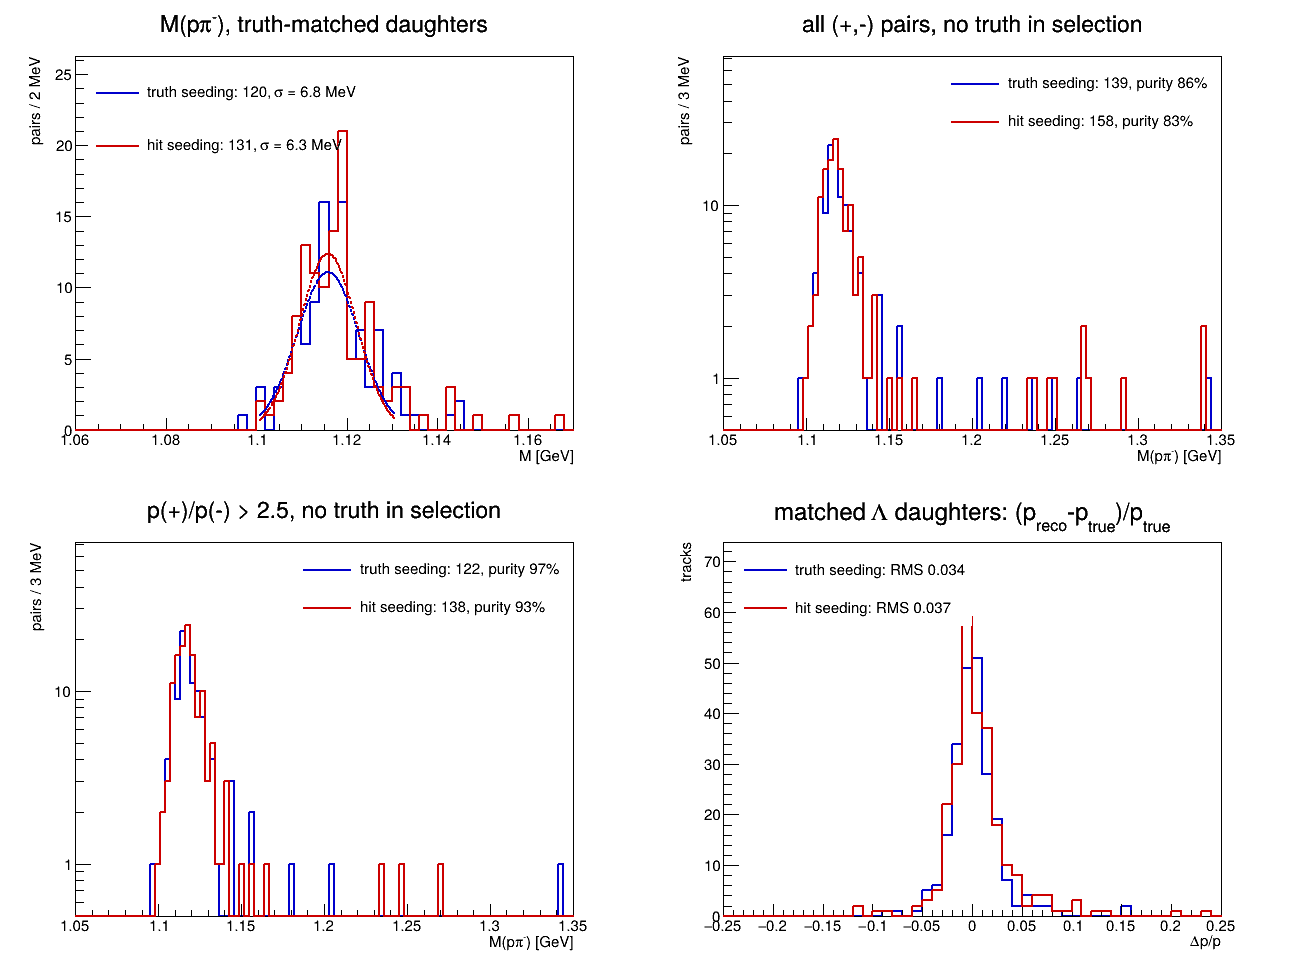
\includegraphics[width=\textwidth]{07_hit_seeding/mass_seeding_compare_new.png}\\
\footnotesize new geometry; blue truth, red hit seeding
\column{0.45\textwidth}\small
\begin{tabular}{@{}lcc@{}}
\toprule
& old & new\\
\midrule
pairs, truth / hit & 210 / 229 & 120 / 131\\
$\sigma$ [MeV], truth / hit & 6.9 / 6.8 & 6.8 / 6.3\\
$\Delta p/p$ RMS & 3.8 / 4.4\,\% & 3.4 / 3.7\,\%\\
\midrule
purity after cut & 86 / \bad{64\,\%} & 97 / 93\,\%\\
$\pm$20\,MeV: sig./cand. & 206 / 219 & 116 / 116\\
\bottomrule
\end{tabular}
\vspace{2mm}
\begin{itemize}\footnotesize
\item Same peak: $M(\text{hit}) - M(\text{truth})$ RMS 4.4\,MeV on common decays
\item Hit seeding also tracks secondaries: ``other'' tracks old 198 $\to$ 432, new 68 $\to$ 91
\item Background matters only in the thick old geometry
\end{itemize}
\end{columns}
\end{frame}

%-------------------------------------------------------------------------------------
\begin{frame}{Correction: per $p\pi^-$ decay vs per generated $\Lambda$}
\begin{columns}[T]
\column{0.5\textwidth}
\small
1000 $\Lambda$, 50--100\,GeV, new geometry:\\[1mm]
\begin{tabular}{@{}lccc@{}}
\toprule
fate & N & $z_{\rm end} < 5.8$\,m & last $z_{\rm end}$\\
\midrule
$p\pi^-$ & 485 & 438 & 8.7\,m\\
$n\pi^0$ & 278 & 246 & 9.4\,m\\
other & 237 & 11 & 12.4\,m\\
\bottomrule
\end{tabular}
\column{0.5\textwidth}
\begin{itemize}\small
\item ``other'' = \textbf{interacted} (all have daughters), 205 at $z = 6$--10\,m; none leaves the world (3 Nov: wrong)
\item A $\Lambda$ not decayed by $\sim$6\,m interacts before it can decay
\item ``90\,\% of $p\pi^-$ decays before B0'' is \textbf{conditional}
\item Per generated $\Lambda$: 68\,\% decay before 5.8\,m vs \textbf{66\,\%} from $1-e^{-L/\lambda}$
\end{itemize}
\end{columns}
\vspace{3mm}
\centering $\Rightarrow$ \textbf{per generated $\Lambda$} is the unbiased denominator
\end{frame}

%-------------------------------------------------------------------------------------
\begin{frame}{$\Lambda$s up to 275\,GeV: expectation}
\begin{itemize}
\item New samples: 100--275\,GeV, 2$\times$500 per geometry, \#3116 build (both seedings)
\item Mean decay length $\lambda = (p/m)\,c\tau = p[\text{GeV}] \times 7.07$\,cm
\item Decays before the B0 ($L = 5.8$\,m): $P = 1 - e^{-L/\lambda}$
\end{itemize}
\centering
\begin{tabular}{@{}lcccc@{}}
\toprule
$p_\Lambda$ & 50\,GeV & 100\,GeV & 200\,GeV & 275\,GeV\\
\midrule
$\lambda$ & 3.5\,m & 7.1\,m & 14\,m & 19\,m\\
decay before B0 & 81\,\% & 56\,\% & 34\,\% & \bad{26\,\%}\\
\bottomrule
\end{tabular}
\begin{itemize}
\item But the $\pi^-$ carries 6--25\,\% of $p_\Lambda$ $\Rightarrow$ \good{no longer soft} at high momentum
\end{itemize}
\end{frame}

%-------------------------------------------------------------------------------------
\begin{frame}{Acceptance and efficiency vs $\Lambda$ momentum (new geometry)}
\centering
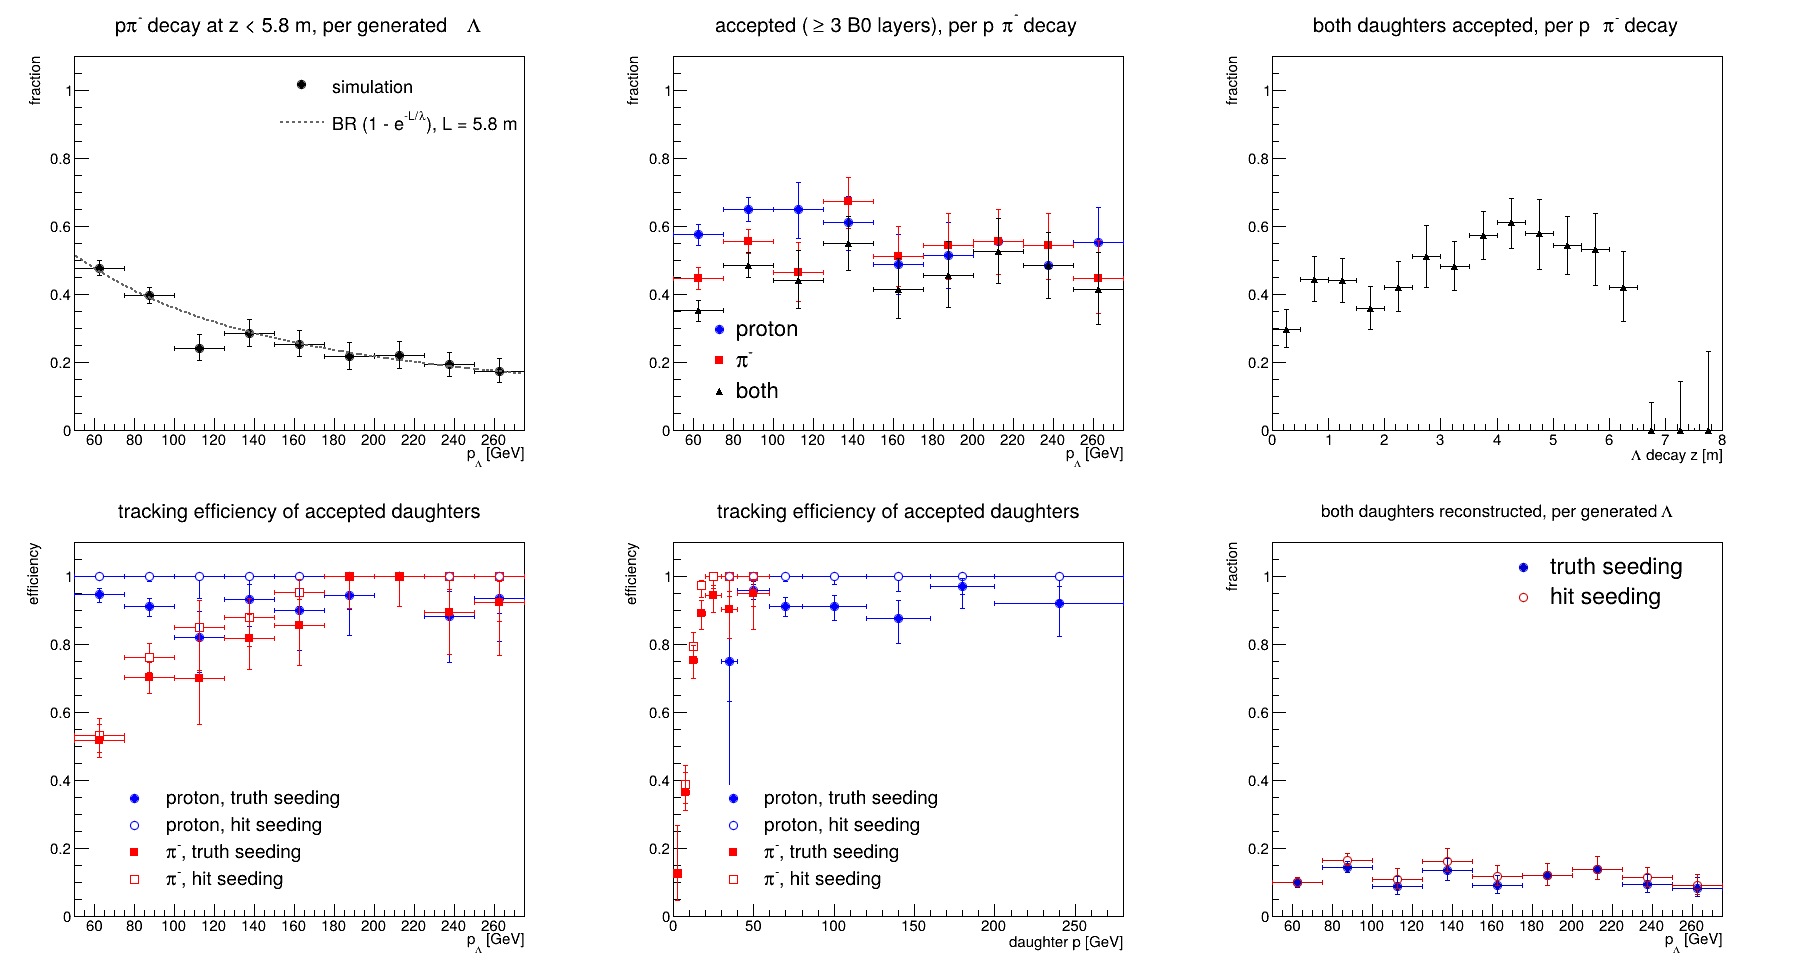
\includegraphics[width=0.88\textwidth]{08_momentum/vs_momentum_new.png}\\
\footnotesize top: $p\pi^-$ decay before B0 (dashed: decay law), acceptance vs $p_\Lambda$, vs decay $z$;
bottom: tracking eff.\ vs $p_\Lambda$ and vs daughter $p$ (filled truth, open hit), both reconstructed per generated $\Lambda$
\end{frame}

%-------------------------------------------------------------------------------------
\begin{frame}{Acceptance and efficiency vs $\Lambda$ momentum (old geometry)}
\centering
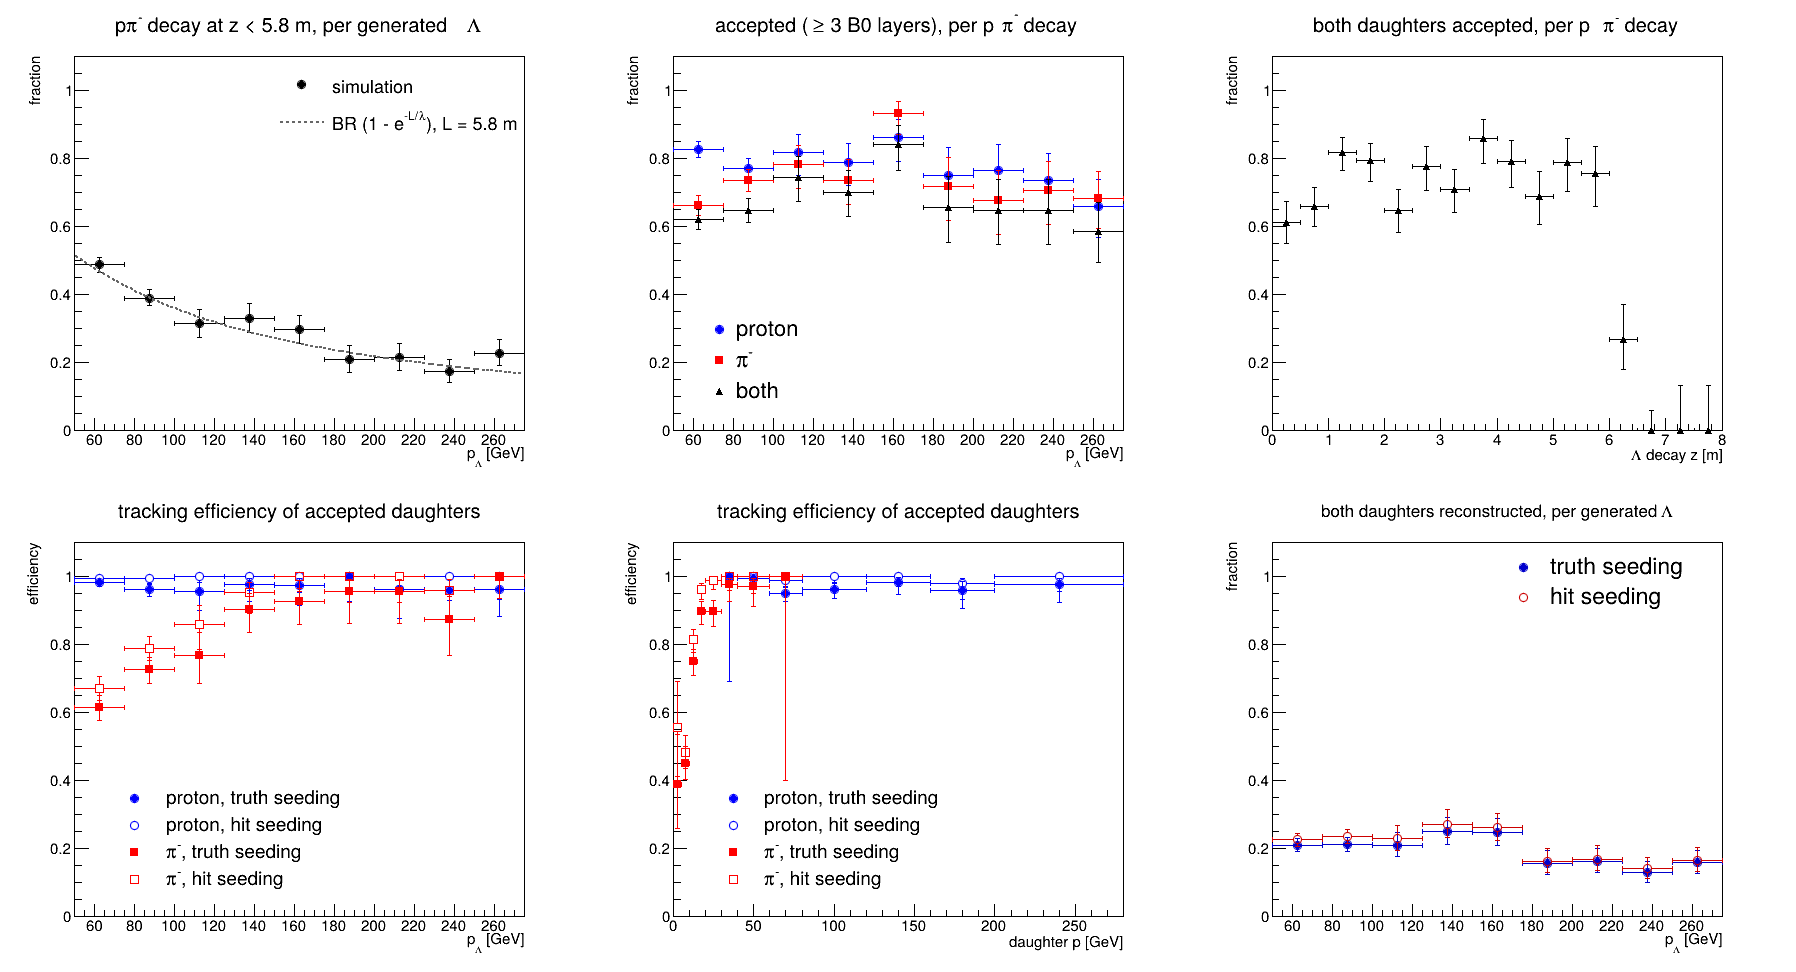
\includegraphics[width=0.88\textwidth]{08_momentum/vs_momentum_old.png}
\end{frame}

%-------------------------------------------------------------------------------------
\begin{frame}{Energetic $\Lambda$s: roughly flat}
\centering\small
\begin{tabular}{@{}lccccc@{}}
\toprule
$p_\Lambda$ [GeV] & $p\pi^-$ decay before B0 & \multicolumn{2}{c}{$\pi^-$ eff., truth / hit} & \multicolumn{2}{c}{\textbf{both rec.\ / generated $\Lambda$}, truth / hit}\\
& (decay law) & old & new & old & new\\
\midrule
50--75 & 48\,\% (47) & 62 / 67\,\% & 52 / 53\,\% & 21 / 23\,\% & 10 / 10\,\%\\
150--175 & 25--30\,\% (25) & 93 / 100\,\% & 86 / 95\,\% & 25 / 26\,\% & 9 / 12\,\%\\
250--275 & 18--23\,\% (17) & 100 / 100\,\% & 93 / 100\,\% & 16 / 17\,\% & 9 / 10\,\%\\
\bottomrule
\end{tabular}
\vspace{2mm}
\begin{itemize}\small
\item Decay before the B0 follows the decay law
\item $\pi^-$ efficiency vs its own momentum: $\approx$40\,\% below 5\,GeV $\to$ $\approx$100\,\% above 20\,GeV
\item Acceptance (both, per decay): old 60--85\,\%, new 35--55\,\% ($\phi$ gap, not momentum); nothing beyond $z \approx 6.5$\,m
\item \textbf{Fewer early decays, but better reconstructed:} new geometry 21\,\% of early decays fully reconstructed at 50--75\,GeV, 40--60\,\% above 150\,GeV
\item 30--55 $p\pi^-$ decays per bin above 100\,GeV: $\pm$5--10 points
\end{itemize}
\end{frame}

%-------------------------------------------------------------------------------------
\begin{frame}{Summary}
\begin{itemize}
\item \textbf{Hit seeding (EICrecon\#3116) works} for displaced $\Lambda$ daughters: seed for every accepted daughter,
every accepted proton reconstructed; \good{13.1\,\%} (new) / 22.9\,\% (old) of all $\Lambda$ fully reconstructed
(truth seeding 12.0 / 21.0\,\%); same mass peak
\item It also tracks secondaries: purity without truth 93\,\% (new), 64\,\% (old, thick sensors)
\item \textbf{Soft-$\pi^-$ loss is in the CKF}, not in the seeding
\item \textbf{5\,keV} is now the default B0 threshold (\#3084)
\item \textbf{Up to 275\,GeV:} fewer $\Lambda$s decay before the B0 (26\,\% at 275\,GeV), but they are reconstructed better $\Rightarrow$
fully reconstructed fraction roughly flat (old 15--25\,\%, new 9--14\,\%)
\item Use \textbf{per generated $\Lambda$}: ``per $p\pi^-$ decay'' is conditional on an early decay
\end{itemize}
\vspace{2mm}
\textbf{Open:} \bad{old-geometry efficiency jump between EICrecon builds}; CKF loss of soft tracks; +2\,MeV mass shift (old geometry);
follow \#3116 until merged; full events with backgrounds and vertexing
\end{frame}

%-------------------------------------------------------------------------------------
\appendix
\begin{frame}{Backup: reproducing}
\small
\begin{itemize}
\item \code{scripts/build/build_eicrecon.sh EICrecon_pr3116 3116}; \code{scripts/build/build_epic.sh epic_43f427e <commit>}
\item \code{scripts/production/lambda_rereco.sh <GEO> <NAME> EICrecon_pr3116 eicreconpr3116}
\item \code{PMIN=100 PMAX=275 SIM_ONLY=1 scripts/production/lambda_sample.sh ...}
\item \code{macros/efficiency/lambda_vs_momentum.C}, \code{macros/mass/lambda_mass_seeding_compare.C}
\item \code{scripts/make_results.sh 07 08}
\end{itemize}
\textbf{Pitfalls}
\begin{itemize}
\item The nightly changes under you: \code{GEO=container} is no longer the old geometry $\Rightarrow$ pin commits
\item JANA keeps the \emph{first} value of a repeated \code{-P} (\code{jana:nevents})
\end{itemize}
\end{frame}

\end{document}
